\documentclass[12pt, titlepage]{article}

\usepackage{fullpage}
\usepackage[round]{natbib}
\usepackage{multirow}
\usepackage{multicol}
\usepackage{booktabs}
\usepackage{tabularx}
\usepackage{graphicx}
\usepackage{float}
\usepackage{hyperref}
\usepackage{svg}
\usepackage{longtable}
\usepackage{pdflscape}
\hypersetup{
    colorlinks,
    citecolor=blue,
    filecolor=black,
    linkcolor=red,
    urlcolor=blue
}

%% Comments

\usepackage{color}

\newif\ifcomments\commentstrue %displays comments
%\newif\ifcomments\commentsfalse %so that comments do not display

\ifcomments
\newcommand{\authornote}[3]{\textcolor{#1}{[#3 ---#2]}}
\newcommand{\todo}[1]{\textcolor{red}{[TODO: #1]}}
\else
\newcommand{\authornote}[3]{}
\newcommand{\todo}[1]{}
\fi

\newcommand{\wss}[1]{\authornote{blue}{SS}{#1}} 
\newcommand{\plt}[1]{\authornote{magenta}{TPLT}{#1}} %For explanation of the template
\newcommand{\an}[1]{\authornote{cyan}{Author}{#1}}

%% Common Parts

\newcommand{\progname}{Software Engineering} % PUT YOUR PROGRAM NAME HERE
\newcommand{\authname}{Team \#22, TeleHealth Insights
\\ Mitchell Weingust
\\ Parisha Nizam
\\ Promish Kandel
\\ Jasmine Sun-Hu} % AUTHOR NAMES                  

\usepackage{hyperref}
    \hypersetup{colorlinks=true, linkcolor=blue, citecolor=blue, filecolor=blue,
                urlcolor=blue, unicode=false}
    \urlstyle{same}
                                


\newcounter{acnum}
\newcommand{\actheacnum}{AC\theacnum}
\newcommand{\acref}[1]{AC\ref{#1}}

\newcounter{ucnum}
\newcommand{\uctheucnum}{UC\theucnum}
\newcommand{\uref}[1]{UC\ref{#1}}

\newcounter{mnum}
\newcommand{\mthemnum}{M\themnum}
\newcommand{\mref}[1]{M\ref{#1}}

\begin{document}

\title{Module Guide for \progname{}} 
\author{\authname}
\date{\today}

\maketitle

\pagenumbering{roman}

\section{Revision History}

\begin{tabularx}{\textwidth}{p{3cm}p{2cm}p{3cm}X}
  \toprule {\bf Date} & {\bf Version} & {\bf Member} & {\bf Notes}\\
  \midrule
  1/13/2025 & 1.0 & Mitchell Weingust & Added 10 - Clinician Dashboard Interfaces\\
  1/13/2025 & 1.1 & Promish Kandel & Added 5 - Module Hierarchy\\
  1/13/2025 & 1.2 & Parisha Nizam & Added 10 - Home Page \\
  1/14/2025 & 1.3 & Parisha Nizam & Added Module Decomposition\\
  1/14/2025 & 1.4 & Jasmine Sun-Hu & Added 7 - Module Decomposition, Anticipated and Unlikely Changes, and User Interfaces\\
  1/14/2025 & 1.5 & Mitchell Weingust & Added 12 - Timeline\\
  1/14/2025 & 1.6 & Mitchell Weingust & Added 10 - Clinician Dashboard FSM\\
  1/14/2025 & 1.7 & Parisha Nizam & Added 8 - Traceability Matrix\\
  1/14/2025 & 1.8 & Mitchell Weingust & Added 7 - Module Decomposition\\
  1/14/2025 & 1.9 & Promish Kandel & Added 9 - Use Hierarchy Between Modules\\
  1/14/2025 & 1.10 & Promish Kandel & Added 7 - Module Decomposition\\
  1/15/2025 & 1.11 & Everyone & FSM Machine and Review \\
  03/23/2025 & 2.0 & Promish Kandel & Implemented TA Feedback: \href{https://github.com/parishanizam/TeleHealth/issues/498}{Added AC3 to account for exact hardware changes}\\
  03/23/2025 & 2.1 & Promish Kandel & Implemented TA Feedback: \href{https://github.com/parishanizam/TeleHealth/issues/499}{Removed input/output devices as these can change, as shown in AC3}\\
  03/23/2025 & 2.2 & Promish Kandel & Implemented TA Feedback: \href{https://github.com/parishanizam/TeleHealth/issues/500}{Updated the wording for UC1 to be more descriptive rather than just "core structure"}\\
  03/23/2025 & 2.3 & Promish Kandel & Implemented TA Feedback: \href{https://github.com/parishanizam/TeleHealth/issues/501}{Removed bilingual as it doesn't matter in the context of unlikely changes}\\
  03/23/2025 & 2.4 & Promish Kandel & Implemented TA Feedback: \href{https://github.com/parishanizam/TeleHealth/issues/502}{AppController was fully removed and replaced with Landing Page GUI which is now a behaviour hinding module.}\\
  03/23/2025 & 2.5 & Promish Kandel & Implemented TA Feedback: \href{https://github.com/parishanizam/TeleHealth/issues/504}{Added a logical module showcase our hardware hiding due to the browser. Also made note that this is an external module, not something we implemented. Show cased in section 7.1 Hardware hiding modules}\\
  03/23/2025 & 2.6 & Promish Kandel & Implemented TA Feedback: \href{https://github.com/parishanizam/TeleHealth/issues/505}{Spelling was fixed} and \href{https://github.com/parishanizam/TeleHealth/issues/506}{wording was made more consistent}\\
  03/23/2025 & 2.7 & Promish Kandel & Implemented TA Feedback: \href{https://github.com/parishanizam/TeleHealth/issues/507}{Section 5 and traceability matrix are hyperlinked. I also fixed the hyperlink to point to the respective module decompostion rather than section 5}\\
  03/23/2025 & 2.8 & Promish Kandel & Implemented TA Feedback: \href{https://github.com/parishanizam/TeleHealth/issues/508}{Module Hierarchy diagram was added as a pdf to allow for zooming in and to make it more clear. This diagram now also contains Landing Page GUI and Logical Module as an external module}\\
  03/23/2025 & 2.9 & Promish Kandel & Implemented TA Feedback: \href{https://github.com/parishanizam/TeleHealth/issues/338}{Update the secrets for 7.2.7 Question Banks Module }\\
  03/23/2025 & 3.0 & Promish Kandel & Removed Logging, RealTimeFeedback and Report Generation modules based on changing design decisions.\\


  \bottomrule
\end{tabularx}

\newpage

\section{Reference Material}

This section records information for easy reference.

\subsection{Abbreviations and Acronyms}

\renewcommand{\arraystretch}{1.2}
\begin{tabular}{l l} 
  \toprule		
  \textbf{symbol} & \textbf{description}\\
  \midrule 
  AC & Anticipated Change\\
  DAG & Directed Acyclic Graph \\
  M & Module \\
  MG & Module Guide \\
  OS & Operating System \\
  R & Requirement\\
  SC & Scientific Computing \\
  SRS & Software Requirements Specification\\
  \progname & Explanation of program name\\
  UC & Unlikely Change \\
  FSM & Finite State Machine \\
  \bottomrule
\end{tabular}\\

\newpage

\tableofcontents

\listoftables

\listoffigures

\newpage

\pagenumbering{arabic}

\section{Introduction}

Decomposing a system into modules is a commonly accepted approach to developing
software.  A module is a work assignment for a programmer or programming
team~\citep{ParnasEtAl1984}.  We advocate a decomposition
based on the principle of information hiding~\citep{Parnas1972a}.  This
principle supports design for change, because the ``secrets'' that each module
hides represent likely future changes.  Design for change is valuable in SC,
where modifications are frequent, especially during initial development as the
solution space is explored.  

Our design follows the rules layed out by \citet{ParnasEtAl1984}, as follows:
\begin{itemize}
\item System details that are likely to change independently should be the
  secrets of separate modules.
\item Each data structure is implemented in only one module.
\item Any other program that requires information stored in a module's data
  structures must obtain it by calling access programs belonging to that module.
\end{itemize}

After completing the first stage of the design, the Software Requirements
Specification (SRS), the Module Guide (MG) is developed~\citep{ParnasEtAl1984}. The MG
specifies the modular structure of the system and is intended to allow both
designers and maintainers to easily identify the parts of the software.  The
potential readers of this document are as follows:

\begin{itemize}
\item New project members: This document can be a guide for a new project member
  to easily understand the overall structure and quickly find the
  relevant modules they are searching for.
\item Maintainers: The hierarchical structure of the module guide improves the
  maintainers' understanding when they need to make changes to the system. It is
  important for a maintainer to update the relevant sections of the document
  after changes have been made.
\item Designers: Once the module guide has been written, it can be used to
  check for consistency, feasibility, and flexibility. Designers can verify the
  system in various ways, such as consistency among modules, feasibility of the
  decomposition, and flexibility of the design.
\end{itemize}

The rest of the document is organized as follows. Section
\ref{SecChange} lists the anticipated and unlikely changes of the software
requirements. Section \ref{SecMH} summarizes the module decomposition that
was constructed according to the likely changes. Section \ref{SecConnection}
specifies the connections between the software requirements and the
modules. Section \ref{SecMD} gives a detailed description of the
modules. Section \ref{SecTM} includes two traceability matrices. One checks
the completeness of the design against the requirements provided in the SRS. The
other shows the relation between anticipated changes and the modules. Section
\ref{SecUse} describes the use relation between modules.

\section{Anticipated and Unlikely Changes} \label{SecChange}

This section lists possible changes to the system. According to the likeliness
of the change, the possible changes are classified into two
categories. Anticipated changes are listed in Section \ref{SecAchange}, and
unlikely changes are listed in Section \ref{SecUchange}.

\subsection{Anticipated Changes} \label{SecAchange}

Anticipated changes are the source of the information that is to be hidden
inside the modules. Ideally, changing one of the anticipated changes will only
require changing the one module that hides the associated decision. The approach
adapted here is called design for change.

\begin{description} 
  \begin{item}[\refstepcounter{acnum} 
    \actheacnum 
    \label{acLanguages}:] The supported languages for the assessments (e.g., adding 
     languages like Spanish, French, etc.). 
  \end{item} 
  \begin{item}[\refstepcounter{acnum} \actheacnum 
    \label{acAssessmentTypes}:] The types of assessments supported (e.g., addition 
    of new assessment types like sentence completion, story-telling, etc.). 
  \end{item} 
  \begin{item}[\refstepcounter{acnum} \actheacnum 
    \label{achardware}:] The exact hardware that is going to be used (e.g., the type of
    microphone, type of camera for video recording). 
  \end{item} 
\end{description}

\subsection{Unlikely Changes} \label{SecUchange}

The module design should be as general as possible. However, a general system is
more complex. Sometimes this complexity is not necessary. Fixing some design
decisions at the system architecture stage can simplify the software design. If
these decision should later need to be changed, then many parts of the design
will potentially need to be modified. Hence, it is not intended that these
decisions will be changed.

\begin{description}
  \begin{item}[\refstepcounter{ucnum} \uctheucnum \label{ucCoreAssessmentStructure}:] The structure of our question bank system and the way questions and their associated audio assets are formatted and organized in our database is designed for long-term stability and is unlikely to change.
  \end{item} 
  \begin{item}[\refstepcounter{ucnum} \uctheucnum \label{ucAssessmentPurpose}:] The 
    primary purpose of the system, which is to assist parents in administering speech 
    assessments for children. 
  \end{item} 
\end{description}

\newpage

\section{Module Hierarchy} \label{SecMH}

This section provides an overview of the module design. Modules are summarized
in a hierarchy decomposed by secrets in Table \ref{TblMH}. The modules listed
below, which are leaves in the hierarchy tree, are the modules that will
actually be implemented.

\begin{multicols}{2}
  \begin{description}
    \item [\mref{mClinicianGUI}:] Clinician GUI Module
    \item [\mref{mParentGUI}:]   Parent GUI Module
    \item [\mref{mAppController}:] Landing Page GUI
    \item [\mref{mAPIGateway}:]  API Gateway Module
    \item [\mref{mAuth}:]        Authentication Module
    \item [\mref{mResultStorage}:] Result Storage Module
    \item [\mref{mMediaProcessing}:] Media Processing Module
    \item [\mref{mQuestionBank}:] Question Bank Module
    \item [\mref{mVideoProcessing}:] Video Processing Module
    \item [\mref{mAudioProcessing}:] Audio Processing Module
    \item [\mref{mEnglishBank}:] English Question Bank Module
    \item [\mref{mMandarinBank}:] Mandarin Question Bank Module
    \item [\mref{mMatchingBank1}:] Matching Question Bank Module
    \item [\mref{mRepetitionBank1}:] Repetition Question Bank Module
  \end{description}
\end{multicols}
  

\section{Connection Between Requirements and Design} \label{SecConnection}

The design of the system is intended to satisfy the requirements developed in
the SRS. In this stage, the system is decomposed into modules. The connection
between requirements and modules is listed in Table~\ref{TblRT}.

\section{Module Decomposition} \label{SecMD}

Modules are decomposed according to the principle of ``information hiding''
proposed by \citet{ParnasEtAl1984}. The \emph{Secrets} field in a module
decomposition is a brief statement of the design decision hidden by the
module. The \emph{Services} field specifies \emph{what} the module will do
without documenting \emph{how} to do it. For each module, a suggestion for the
implementing software is given under the \emph{Implemented By} title. If the
entry is \emph{OS}, this means that the module is provided by the operating
system or by standard programming language libraries.  \emph{\progname{}} means the
module will be implemented by the \progname{} software.

Only the leaf modules in the hierarchy have to be implemented. If a dash
(\emph{--}) is shown, this means that the module is not a leaf and will not have
to be implemented.

\begin{table}[h!]
  \centering
  \begin{tabular}{p{0.3\textwidth} p{0.6\textwidth}}
  \toprule
  \textbf{Level 1} & \textbf{Level 2}\\
  \midrule
  
  {Hardware-Hiding} & Logical module \\
  \midrule
  
  \multirow{8}{0.3\textwidth}{Behaviour-Hiding} & Clinician GUI\\
  & Parent GUI\\
  & Landing Page GUI\\
  & Authentication Module\\
  & Result Storage Module\\
  & Real-Time Feedback Module\\ 
  & Report Generation Module\\
  & Media Processing Module\\
  & Video Processing Module\\
  & Audio Processing Module\\
  & Logging Module\\
  & Question Bank Module\\
  & Mandarin Question Bank\\
  & English Question Bank\\
  & Repetition Question Bank Module\\
  & Matching Question Bank Module\\
  \midrule
  
  \multirow{1}{0.3\textwidth}{Software Decision} & API Gateway\\
  \bottomrule
  
  \end{tabular}
  \caption{Module Hierarchy}
  \label{TblMH}
  \end{table}
  \newpage

\subsection{Hardware Hiding Modules}
 \subsubsection{Logical module}
\begin{description}
  \item[Secrets:]
    This logical module is handled by the browser, which is outside the scope of our project.
    The browser internally manages and isolates both audio and microphone feeds from direct access.
  \item[Services:]
    Although not part of our implementation, the browser ultimately supplies audio and microphone data
    to the Parent GUI (\mref{mParentGUI}) when a user is taking a test.
  \item[Implemented By:]
    Standard web browser
  \item[Type of Module:]
    External 
\end{description}
\subsection{Behaviour-Hiding Module}

\refstepcounter{mnum}
\subsubsection{Clinician GUI (\mthemnum)}
\label{mClinicianGUI}
\begin{description}
\item[Secrets:]The interactive and visual components that allow Clinicians to interact with the system, through the Landing Page GUI (\mref{mAppController}),
               to access patient data and information, and make informed decisions.
\item[Services:]To show application functionality to clinicians, accepting user inputs (choosing assessments to review,
                flagging bias questions) and displaying outputs (assessment summaries).
\item[Implemented By:] ClinicianFrontEnd
\item[Type of Module:] Library
\end{description}

\refstepcounter{mnum}
\subsubsection{Parent GUI (\mref{mParentGUI})}
\label{mParentGUI}

\begin{description}
\item[Secrets:]The interactive and visual components that allow Parents to interact with the system, through the Landing Page GUI (\mref{mAppController}),
               to set up and engage in the assessment with their child.
\item[Services:] To show application functionality to parents, accepting user inputs (selecting answers to questions,
                 completing set up) and displaying outputs (question visuals, button selections).
\item[Implemented By:] ParentFrontEnd
\item[Type of Module:] Library
\end{description}

\refstepcounter{mnum}
\subsubsection{Landing Page GUI (\mref{mAppController})}
\label{mAppController}
  
\begin{description}
  \item[Secrets:]The interactions between the GUIs (\mref{mClinicianGUI}, \mref{mParentGUI}) and the API Gateway (\mref{mAPIGateway}), acting as a means to interface with the software modules.
  \item[Services:]Enables the user to pass information from the GUIs to the backend services.
  \item[Implemented By:] AppController
  \item[Type of Module:] Library
  \end{description}


\refstepcounter{mnum}
\subsubsection{Authentication Module (\mref{mAuth})}
\label{mAuth}

\begin{description}
\item[Secrets:] The data structures and algorithms used to securely store, validate, and manage user credentials.
\item[Services:] Provides user registration, login, and session management services. Ensures authentication for all system users (parents, clinicians, and admins) to maintain system security.
\item[Implemented By:] AuthenticationService
\item[Type of Module:] Library, Abstract Data Type
\end{description}

\refstepcounter{mnum}
\subsubsection{Result Storage Module (\mref{mResultStorage})}
\label{mResultStorage}

\begin{description}
\item[Secrets:] The schema and mechanisms used to store, index, and retrieve assessment results and metadata efficiently.
\item[Services:] Manages the storage and retrieval of processed media flags, assessment results, and associated metadata. Ensures data security and organization to support reporting and feedback functionalities.
\item[Implemented By:] ResultStorageService
\item[Type of Module:] Record, Abstract Object
\end{description}

\refstepcounter{mnum}
\subsubsection{Media Processing Module (\mref{mMediaProcessing})}
\label{mMediaProcessing}

\begin{description}
\item[Secrets:] The design and implementation of how media (video and audio) is processed in the system.
\item[Services:] Provides high-level functionality for media processing by delegating tasks to its submodules: Video Processing Module and Audio Processing Module. Acts as an abstraction layer for handling media data.
\item[Implemented By:] Media-processing-service
\item[Type of Module:]  Abstract Object
\end{description}

\refstepcounter{mnum}
\subsubsection{Question Bank Module (\mref{mQuestionBank})}
\label{mQuestionBank}

\begin{description}
\item[Secrets:] Maintains all question bank submodules and the internal logic for routing each request to the appropriate submodule.
\item[Services:]Acts as a facade to provide unified access to all question banks.
This module handles requests for retrieving, adding, updating, or delegating questions 
to appropriate submodules.
\item[Implemented By:] QuestionBankService
\item[Type of Module:] Abstract Object
\end{description}

\refstepcounter{mnum}
\subsubsection{Video Processing Module (\mref{mVideoProcessing})}
\label{mVideoProcessing}

\begin{description}
\item[Secrets:] The methods and algorithms used to process video data, including frame extraction, format handling, and metadata processing.
\item[Services:] Handles all video-related data processing tasks, such as analyzing video frames, ensuring quality, and extracting relevant details. This module communicates with the Media Processing Module.
\item[Implemented By:] Media-processing-service
\item[Type of Module:]  Abstract Object
\end{description}

\refstepcounter{mnum}
\subsubsection{Audio Processing Module (\mref{mAudioProcessing})}
\label{mAudioProcessing}
\begin{description}
\item[Secrets:] The methods and algorithms used to process audio data, such as format conversions, noise filtering, and speech analysis.
\item[Services:] Handles all audio-related data processing tasks, including speech detection, sound quality analysis, and extracting key audio features. This module communicates with the Media Processing Module.
\item[Implemented By:] Media-processing-service
\item[Type of Module:] Abstract Object
\end{description}

\refstepcounter{mnum}
\subsubsection{English Question Bank Module (\mref{mEnglishBank})}
\label{mEnglishBank}

\begin{description}
\item[Secrets:]The format for storing, tagging and/or indexing English questions
\item[Services:]Converts the input data into the data structure used by the
  input parameters module.
\item[Implemented By:] EnglishQuestionManager
\item[Type of Module:] Abstract Data Type
\end{description}

\refstepcounter{mnum}
\subsubsection{Mandarin Question Bank Module (\mref{mMandarinBank})}
\label{mMandarinBank}

\begin{description}
\item[Secrets:]The format and structure of the input data.
\item[Services:]Converts the input data into the data structure used by the
  input parameters module.
\item[Implemented By:] MandarinQuestionManager
\item[Type of Module:] Abstract Data Type
\end{description}

\refstepcounter{mnum}
\subsubsection{Matching Question Bank Module (\mref{mMatchingBank1})}
\label{mMatchingBank1}

\begin{description}
\item[Secrets:]The format and structure of the input data.
\item[Services:]Converts the input data into the data structure used by the
  input parameters module.
\item[Implemented By:] MatchingQuestionService
\item[Type of Module:] Library
\end{description}

\refstepcounter{mnum}
\subsubsection{Repetition Question Bank Module (\mref{mRepetitionBank1})}
\label{mRepetitionBank1}

\begin{description}
\item[Secrets:]The format and structure of the input data.
\item[Services:]Converts the input data into the data structure used by the
  input parameters module.
\item[Implemented By:] MatchingQuestionService
\item[Type of Module:] Library
\end{description}

\subsection{Software Decision Module}

    \refstepcounter{mnum}
    \subsubsection{API Gateway Module (\mref{mAPIGateway})}
    \label{mAPIGateway}
  
    \begin{description}
      \item[Secrets:]The interactions between the Landing Page GUI (\mref{mAppController}) and the inter-dependencies of all other software modules, including inherited modules (
      \mref{mResultStorage},
      \mref{mMediaProcessing},
      \mref{mQuestionBank},
      \mref{mAudioProcessing},
      \mref{mEnglishBank},
      \mref{mMandarinBank},
      \mref{mMatchingBank1},
      \mref{mRepetitionBank1}).
      \item[Services:]Enables the user to access the system and interact with its components, consisting of the Patient, Client, and Admin views.
      \item[Implemented By:] APIGateway
      \item[Type of Module:] Library
      \end{description}

\section{Traceability Matrix} \label{SecTM}

This section shows two traceability matrices: between the modules and the
requirements and between the modules and the anticipated changes.

\begin{table}[H]
  \centering
  \begin{tabular}{p{0.2\textwidth} p{0.6\textwidth}}
  \toprule
  \textbf{Req.} & \textbf{Modules}\\
  \midrule
  
  FR-A1 & \mref{mClinicianGUI}, \mref{mParentGUI}, \mref{mAppController}, \mref{mAuth}, \mref{mQuestionBank}\\
  FR-A2 & \mref{mParentGUI}, \mref{mAppController}, \mref{mAuth}, \mref{mQuestionBank}\\
  FR-A3 & \mref{mClinicianGUI}, \mref{mAppController}, \mref{mAuth}, \mref{mQuestionBank}\\
  FR-A4 & \mref{mAuth}, \mref{mQuestionBank}\\
  FR-A5 & \mref{mAuth}, \mref{mQuestionBank}\\
  
  FR-SS1 & \mref{mParentGUI}, \mref{mAppController}\\
  FR-SS2 & \mref{mParentGUI}, \mref{mAppController}\\
  FR-SS3 & \mref{mParentGUI}, \mref{mAppController}\\
  FR-SS4 & \mref{mParentGUI}, \mref{mAppController}\\
  FR-SS5 & \mref{mParentGUI}, \mref{mAppController}, \mref{mVideoProcessing}\\
  
  FR-AI1 & \mref{mParentGUI}, \mref{mAppController}, \mref{mMediaProcessing}, \mref{mVideoProcessing}, 
           \mref{mMandarinBank}, \mref{mMatchingBank1}, \mref{mRepetitionBank1}\\
  FR-AI2 & \mref{mParentGUI}, \mref{mAppController}, \mref{mAPIGateway}, \mref{mMediaProcessing}, 
           \mref{mVideoProcessing}, \mref{mMandarinBank}, \mref{mMatchingBank1}, \mref{mRepetitionBank1}\\
  FR-AI3 & \mref{mParentGUI}, \mref{mAppController}, \mref{mAPIGateway}, \mref{mMediaProcessing}, 
           \mref{mVideoProcessing}, \mref{mMandarinBank}, \mref{mMatchingBank1}, \mref{mRepetitionBank1}\\
  FR-AI4 & \mref{mParentGUI}, \mref{mAppController}, \mref{mAPIGateway}, \mref{mMediaProcessing}, 
           \mref{mVideoProcessing}, \mref{mMandarinBank}, \mref{mMatchingBank1}, \mref{mRepetitionBank1}\\
  FR-AI5 & \mref{mParentGUI}, \mref{mAppController}, \mref{mAPIGateway}, \mref{mMediaProcessing}, 
           \mref{mVideoProcessing}, \mref{mMandarinBank}, \mref{mMatchingBank1}, \mref{mRepetitionBank1}\\
  FR-AI6 & \mref{mParentGUI}, \mref{mAppController}, \mref{mAPIGateway}, \mref{mResultStorage}, 
           \mref{mMediaProcessing}, \mref{mVideoProcessing}, \mref{mMandarinBank}, \mref{mMatchingBank1}, 
           \mref{mRepetitionBank1}\\
  FR-AI7 & \mref{mParentGUI}, \mref{mAppController}, \mref{mAPIGateway}, \mref{mMediaProcessing}, 
           \mref{mVideoProcessing}, \mref{mMandarinBank}, \mref{mMatchingBank1}, \mref{mRepetitionBank1}\\
  
  FR-DSC1 & \mref{mAPIGateway}, \mref{mResultStorage}, \mref{mQuestionBank}\\
  FR-DSC2 & \mref{mAPIGateway}, \mref{mResultStorage}, \mref{mMediaProcessing}, 
            \mref{mAudioProcessing}, \mref{mMandarinBank}, \mref{mMatchingBank1}\\
  FR-DSC3 & \mref{mAPIGateway}, \mref{mAuth}\\
  FR-DSC4 & \mref{mAPIGateway}, \mref{mAuth}\\
  FR-DSC5 & \mref{mAPIGateway}, \mref{mQuestionBank}, \mref{mAudioProcessing}, \mref{mEnglishBank}\\
  
  FR-VADA1 & \mref{mAPIGateway}, \mref{mMediaProcessing}, \mref{mMandarinBank}, \mref{mMatchingBank1}\\
  FR-VADA2 & \mref{mAPIGateway}, \mref{mMediaProcessing}, \mref{mQuestionBank},
             \mref{mMandarinBank}, \mref{mMatchingBank1}\\
  FR-VADA3 & \mref{mAPIGateway}, \mref{mMediaProcessing}, \mref{mQuestionBank}, 
             \mref{mMandarinBank}, \mref{mMatchingBank1}\\
  
  FR-DPD1 & \mref{mAPIGateway}, \mref{mResultStorage}, \mref{mQuestionBank},
            \mref{mAudioProcessing}, \mref{mEnglishBank}\\
  FR-DPD2 & \mref{mAPIGateway}, \mref{mResultStorage}, \mref{mQuestionBank},
            \mref{mAudioProcessing}, \mref{mEnglishBank}\\
  FR-DPD3 & \mref{mClinicianGUI}, \mref{mAPIGateway}, \mref{mResultStorage},
            \mref{mQuestionBank}, \mref{mAudioProcessing}, \mref{mEnglishBank}\\
  FR-DPD4 & \mref{mClinicianGUI}, \mref{mAPIGateway}, \mref{mResultStorage},
            \mref{mQuestionBank}, \mref{mAudioProcessing}, \mref{mEnglishBank}\\
  
  \bottomrule
  \end{tabular}
  \caption{Trace Between Requirements and Modules}
  \label{TblRT}
  \end{table}
  
  

\begin{table}[H]
\centering
\begin{tabular}{p{0.2\textwidth} p{0.6\textwidth}}
\toprule
\textbf{AC} & \textbf{Modules}\\
\midrule
AC1 & \mref{mVideoProcessing}, \mref{mRepetitionBank1} \\
AC2 & \mref{mVideoProcessing}, \mref{mMatchingBank1}, \mref{mRepetitionBank1} \\
AC3 & \mref{mParentGUI}\\
\end{tabular}
\caption{Trace Between Anticipated Changes and Modules}
\label{TblACT}
\end{table}


\section{Use Hierarchy Between Modules} \label{SecUse}

In this section, the uses hierarchy between modules is
provided. \citet{Parnas1978} said of two programs A and B that A {\em uses} B if
correct execution of B may be necessary for A to complete the task described in
its specification. That is, A {\em uses} B if there exist situations in which
the correct functioning of A depends upon the availability of a correct
implementation of B.  Figure \ref{FigUH} illustrates the use relation between
the modules. It can be seen that the graph is a directed acyclic graph
(DAG). Each level of the hierarchy offers a testable and usable subset of the
system, and modules in the higher level of the hierarchy are essentially simpler
because they use modules from the lower levels.

\begin{figure}[H]
  \centering
  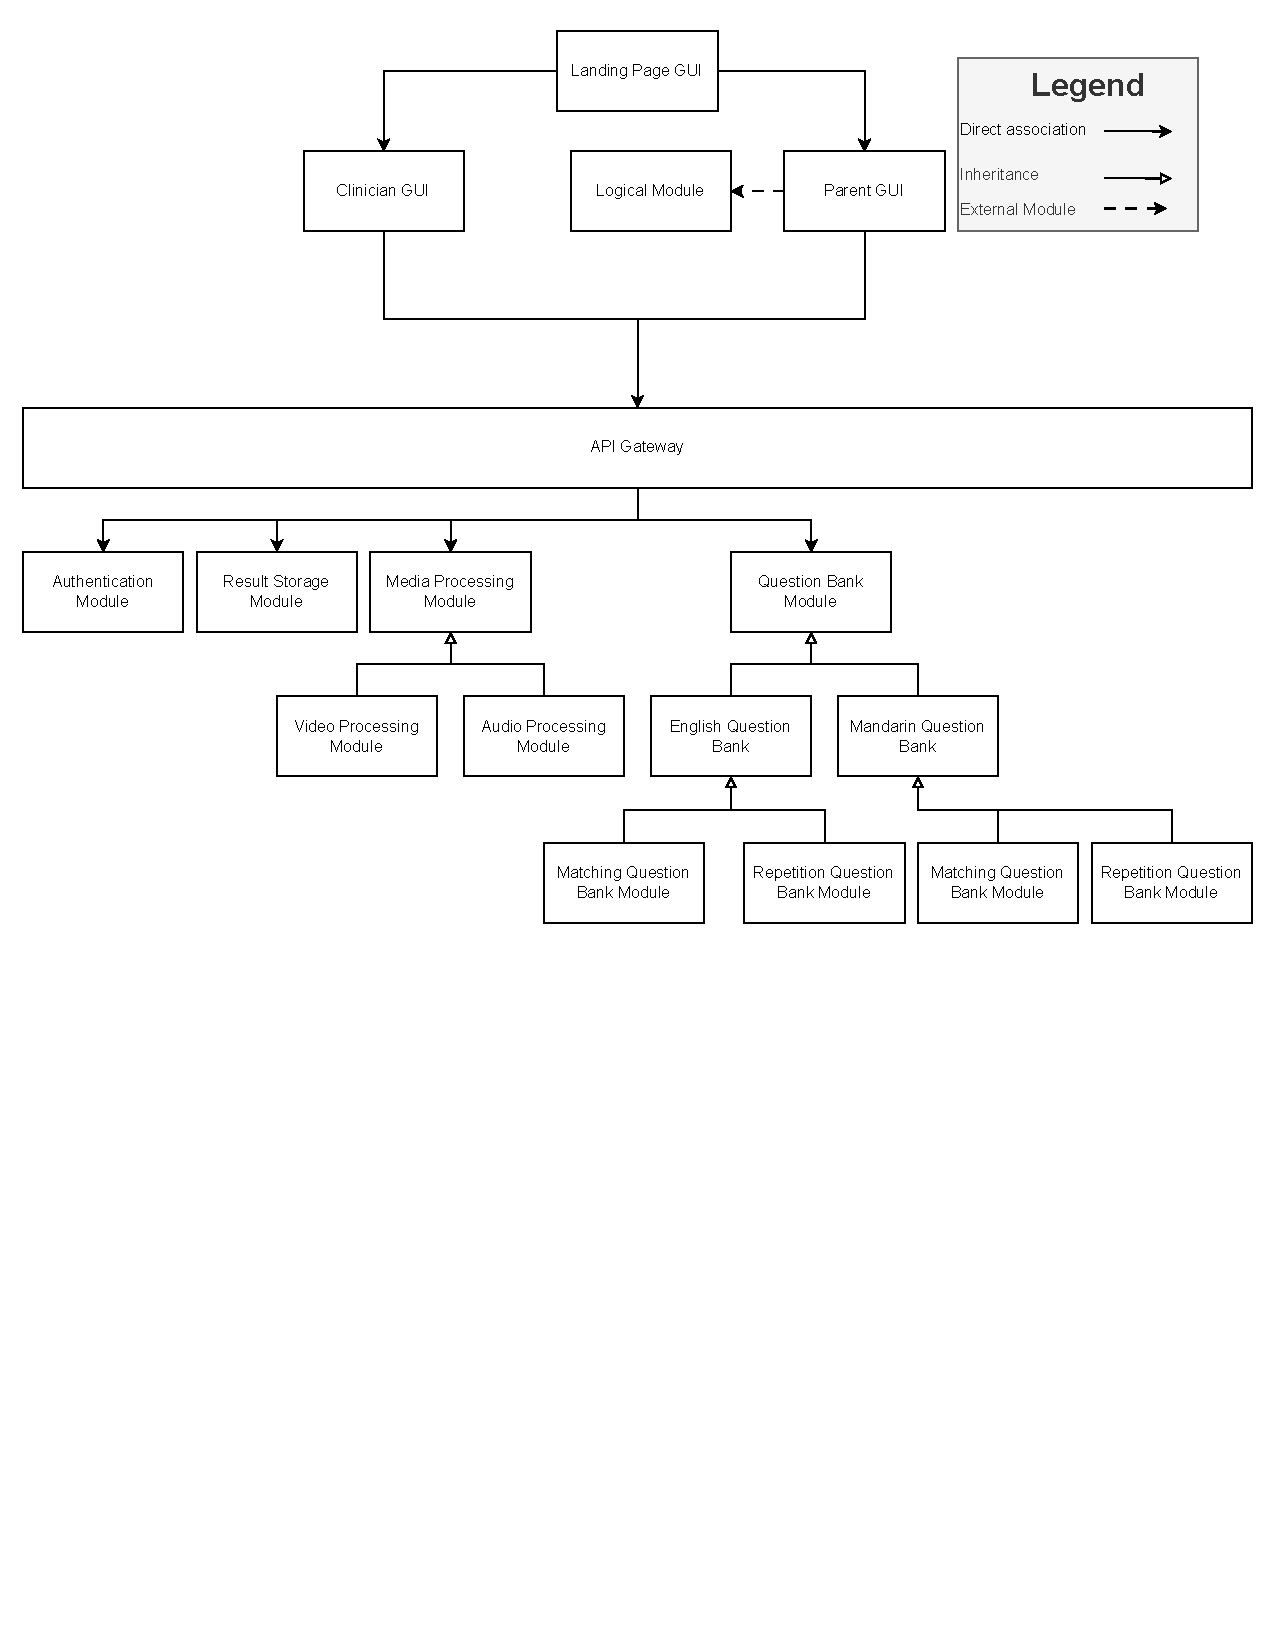
\includegraphics[scale=0.8]{images/ModuleHierachy.pdf}
  \caption{Use hierarchy among modules}
  \label{FigUH}
\end{figure}

%\section*{References}

\newpage

\section{User Interfaces}

\hspace{1.5em}The interface below depicts the initial interface a clinician would see upon logging into their account in the system.
\begin{figure}[H]
  \centering
  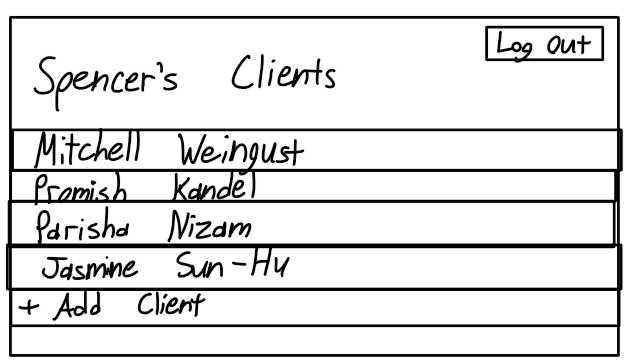
\includegraphics[scale=0.9]{images/Clinician-Dashboard.png}
  \caption{Clinician Dashboard}
\end{figure}

\hspace{1.5em}The interface below depicts the interface a clinician would see upon selecting the Add Client button on the previous Clinician Dashboard screen.
\begin{figure}[H]
  \centering
  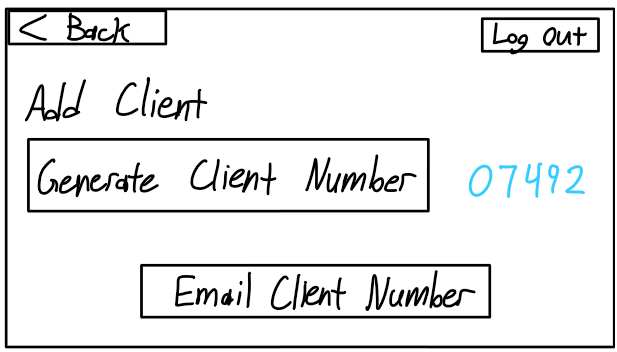
\includegraphics[scale=0.9]{images/Add-Client.png}
  \caption{Add Client}
\end{figure}

\hspace{1.5em}The interface below depicts the patient overview, which can be reached from the Clinician Dashboard by selecting a name from the client list.
\begin{figure}[H]
  \centering
  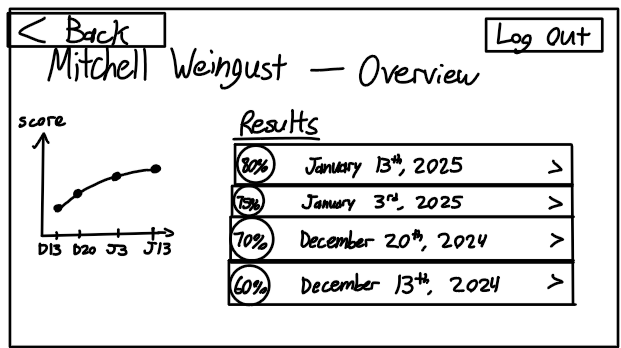
\includegraphics[scale=0.9]{images/Patient-Overview.png}
  \caption{Patient Overview}
\end{figure}

\hspace{1.5em}The interface below depicts the patient assessment results analysis, which can be reached from the Patient Overview by selecting an assessment date from the list of assessments.
\begin{figure}[H]
  \centering
  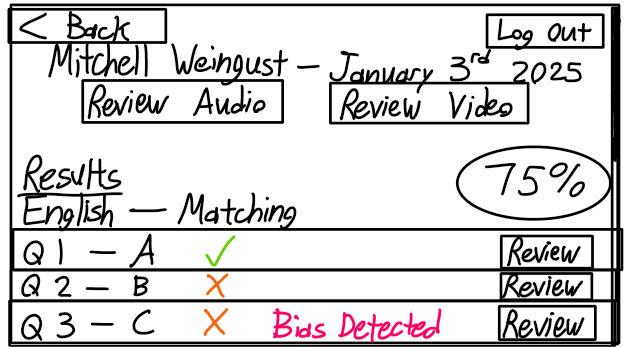
\includegraphics[scale=0.9]{images/Patient-Assessment-Results-Analysis-1.png}
  \caption{Patient Assessment Results Analysis (1)}
\end{figure}

\hspace{1.5em}The interface below depicts a continuation of the patient assessment results analysis, which can be reached from the previous figure, by scrolling the scrollbar on the right edge of the screen.
\begin{figure}[H]
  \centering
  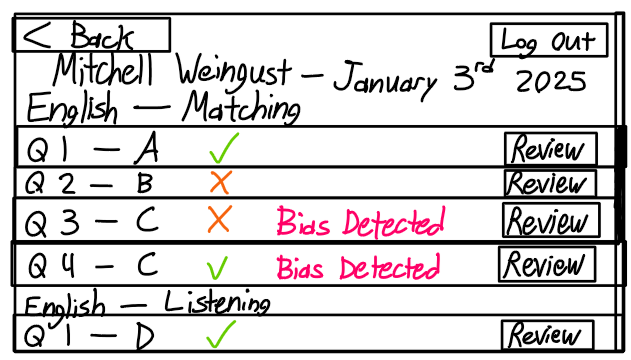
\includegraphics[scale=0.9]{images/Patient-Assessment-Results-Analysis-2.png}
  \caption{Patient Assessment Results Analysis (2)}
\end{figure}

\hspace{1.5em}The interface below depicts the bias review, which can be reached from the Patient Assessment Results Analysis by selecting Review on any of the questions on an assessment.
\begin{figure}[H]
  \centering
  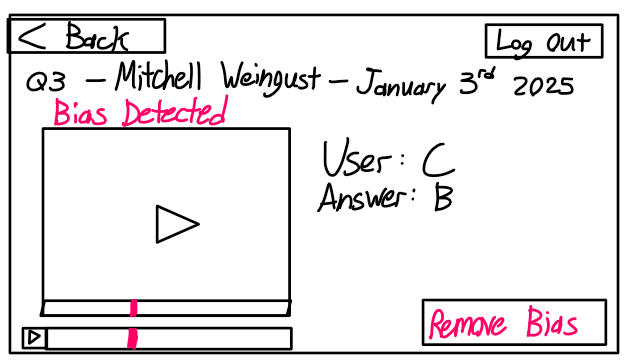
\includegraphics[scale=0.9]{images/Review-Bias.png}
  \caption{Bias Review}
\end{figure}

\hspace{1.5em}The interface below depicts a question review page, where no bias has been detected. The ability to Flag Bias is present in the bottom right corner, to give the Clinician the ability to manually reflect bias in a question.
\begin{figure}[H]
  \centering
  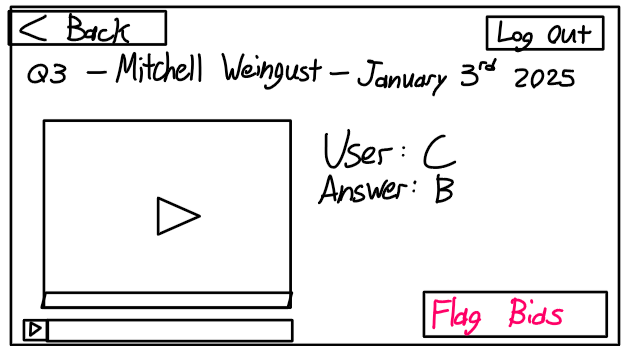
\includegraphics[scale=0.9]{images/Flag-Bias.png}
  \caption{Flag Bias}
\end{figure}

\hspace{1.5em}The interfaces below depicts the interface allowing a user who enters the application to either login to the platform if they have an existing account, or create a new account for new users.
\begin{figure}[H]
  \centering
  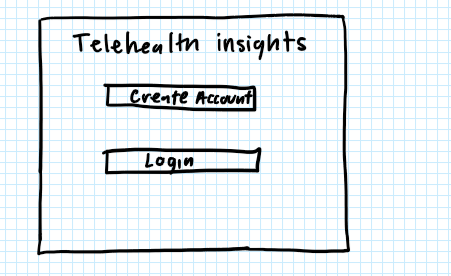
\includegraphics[scale=0.9]{images/createORlogin.png}
  \caption{Login or Create an Account}
\end{figure}

\hspace{1.5em}The interfaces below depicts the flow of selecting which account type to create. If a parent account is chosen, they are able to create a username and password and enter client number to complete the account creation. A clinician account information with be created and provided to the clinician by the admin.
\begin{figure}[H]
  \centering
  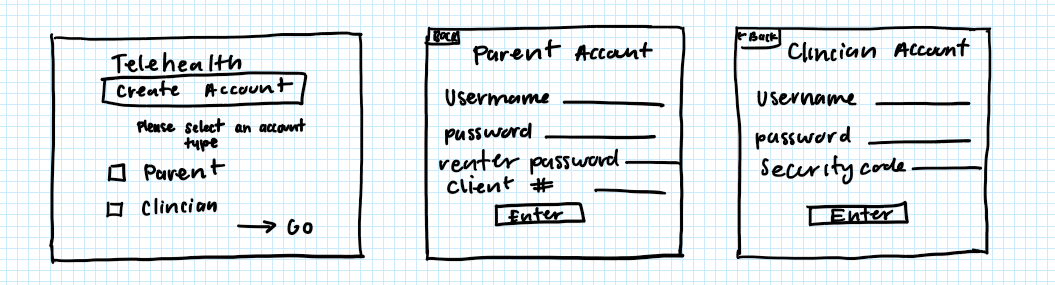
\includegraphics[scale=0.8]{images/create account.png}
  \caption{Create an Account}
\end{figure}

\hspace{1.5em}The interface below depicts the login page overview, where a user can login to the application if they already have an existing account.
\begin{figure}[H]
  \centering
  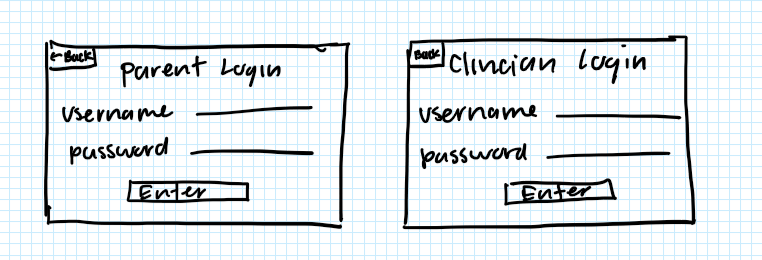
\includegraphics[scale=0.9]{images/loginaccount.png}
  \caption{Login in to account}
\end{figure}

\hspace{1.5em}The interface below depicts the home page for the parent to enter the assesement platform. The home page provides options to learn how to use the assessment platform or start the assessment. 
\begin{figure}[H]
  \centering
  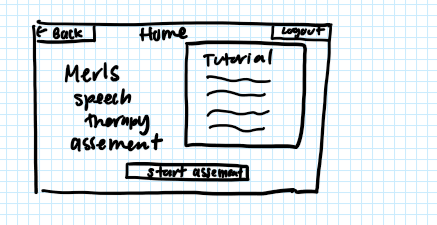
\includegraphics[scale=0.9]{images/homepage.png}
  \caption{Parent HomePage}
\end{figure}

\begin{figure}[H]
  \centering
  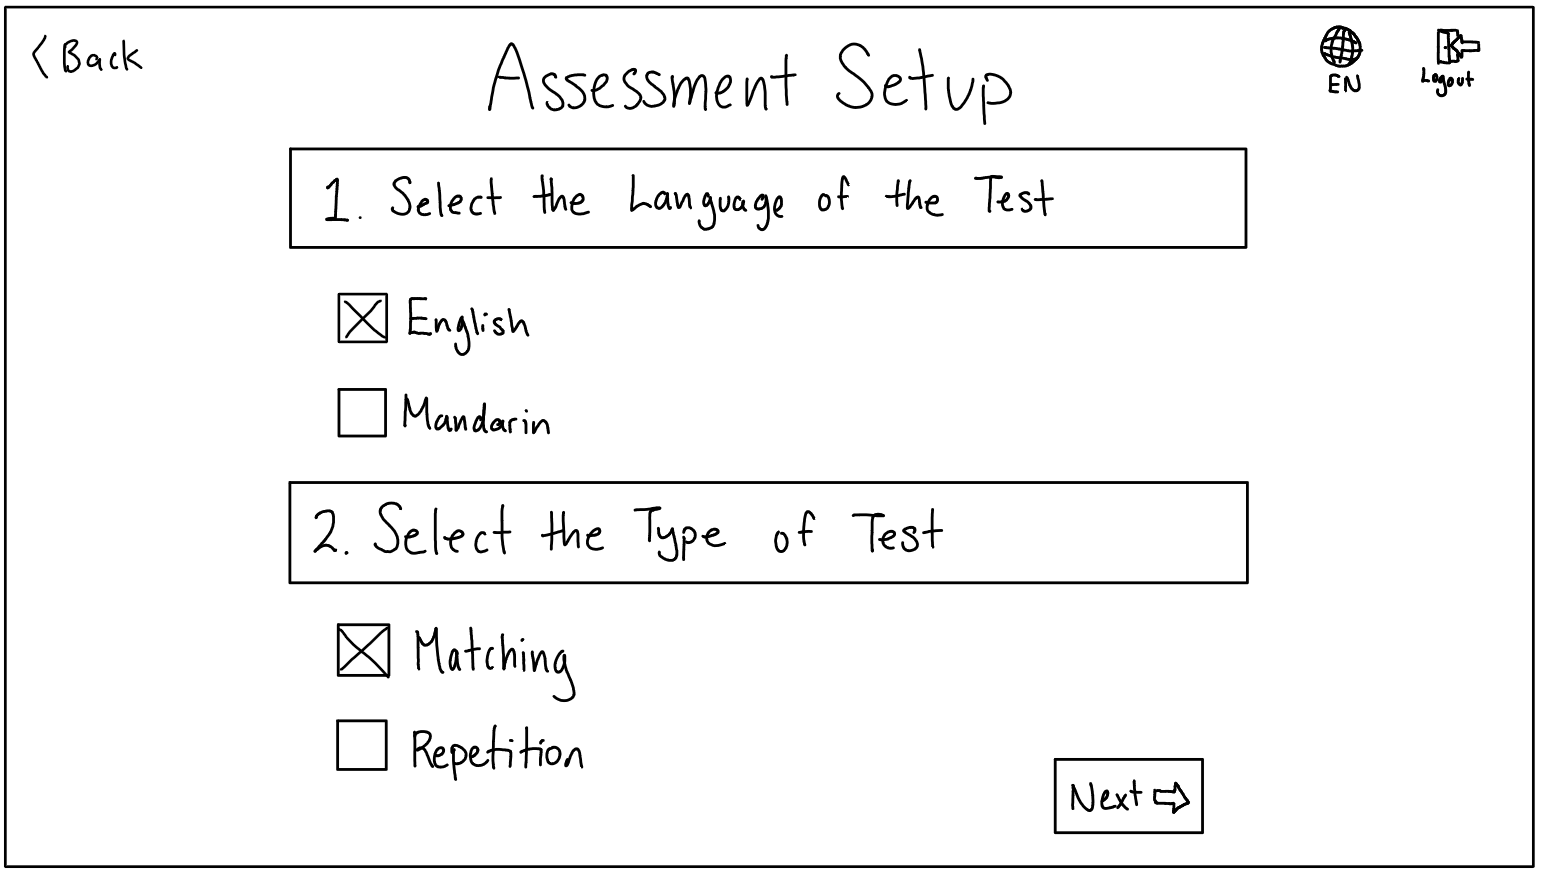
\includegraphics[width=0.75\textwidth]{images/TestSelection.png}
  \caption{Sketch of Assessment Selection Page}
  \label{FigTS}
\end{figure}

\begin{figure}[H]
  \centering
  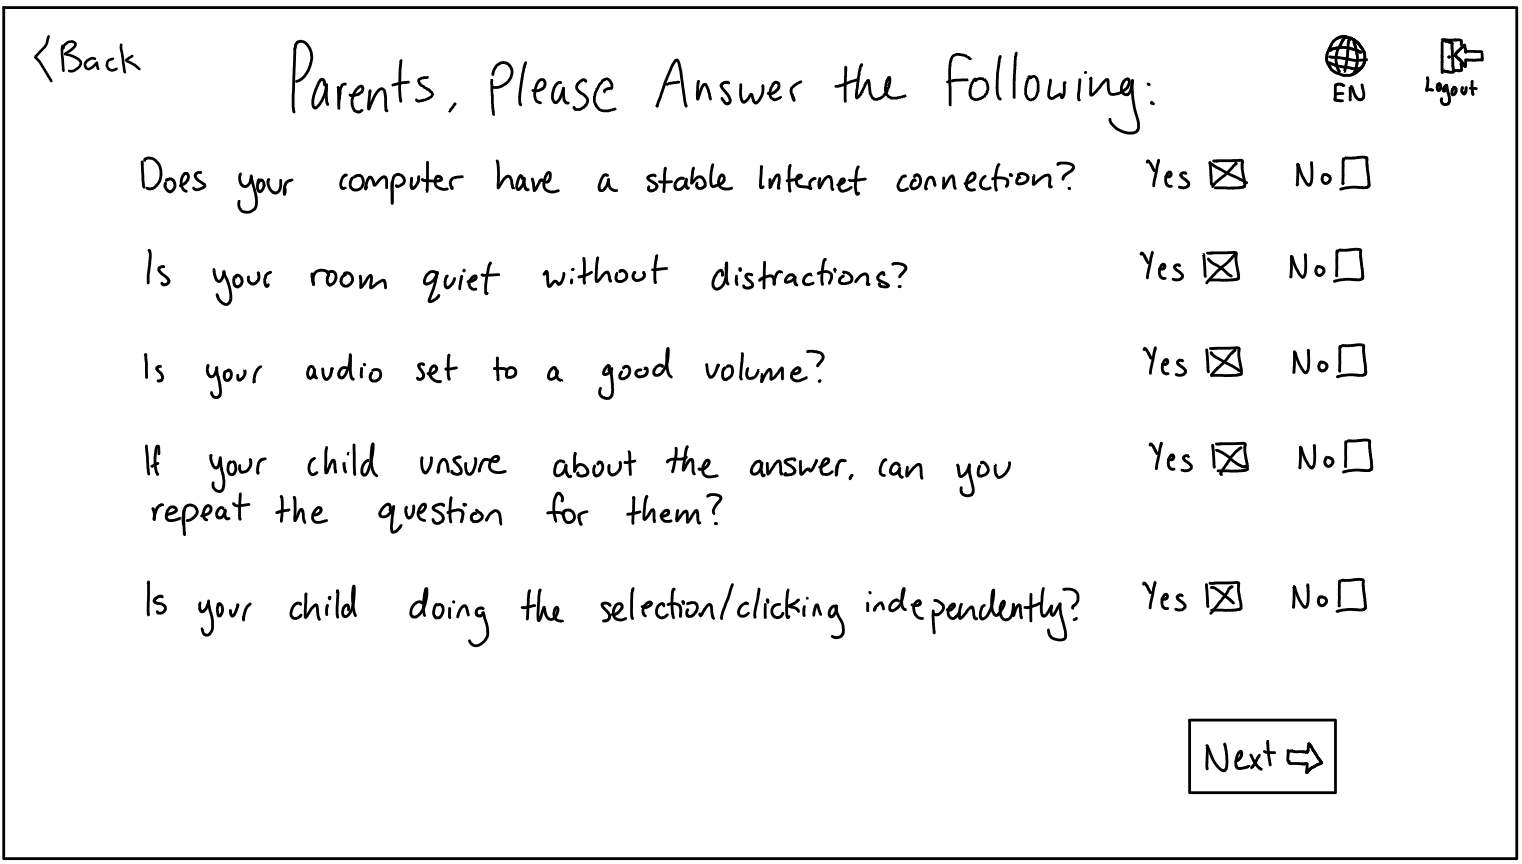
\includegraphics[width=0.75\textwidth]{images/ParentChecklist.png}
  \caption{Sketch of Parent Checklist Page}
  \label{figPC}
\end{figure}

\begin{figure}[H]
  \centering
  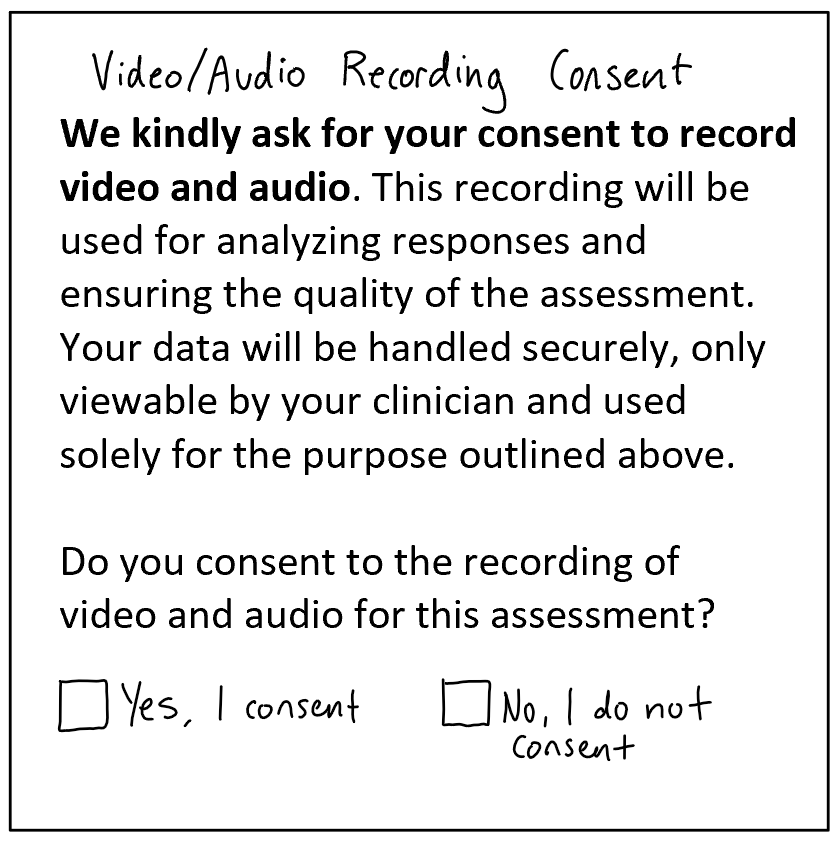
\includegraphics[width=0.5\textwidth]{images/ConsentPopup.png}
  \caption{Sketch of Consent Popup}
  \label{figCP}
\end{figure}

\begin{figure}[H]
  \centering
  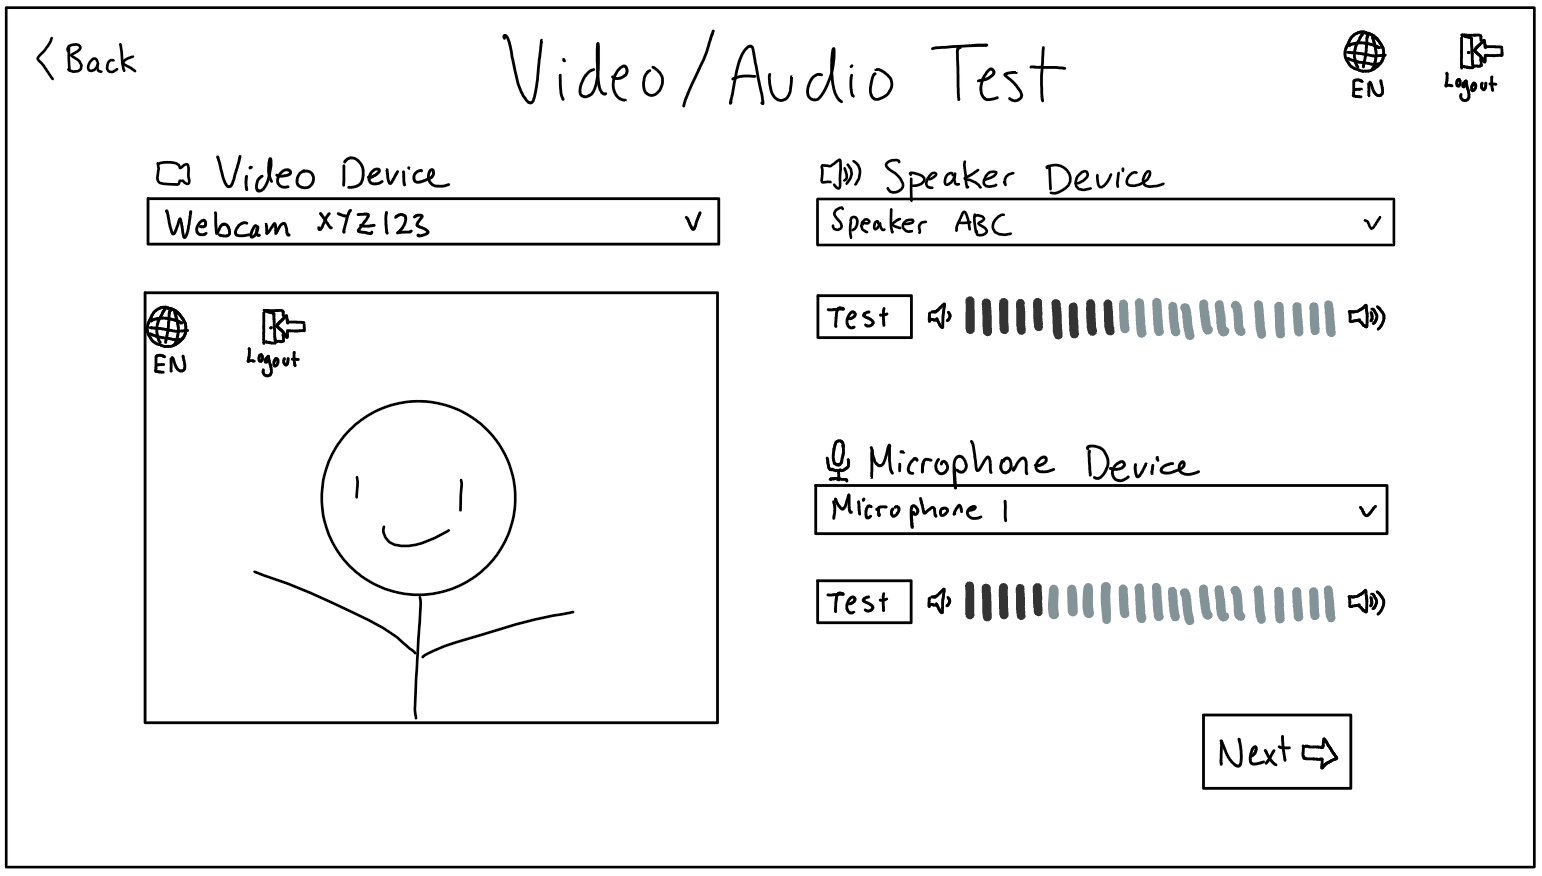
\includegraphics[width=0.75\textwidth]{images/SetupTest.png}
  \caption{Sketch of Video Audio and Mic Test Page}
  \label{figVA}
\end{figure}

\begin{figure}[H]
  \centering
  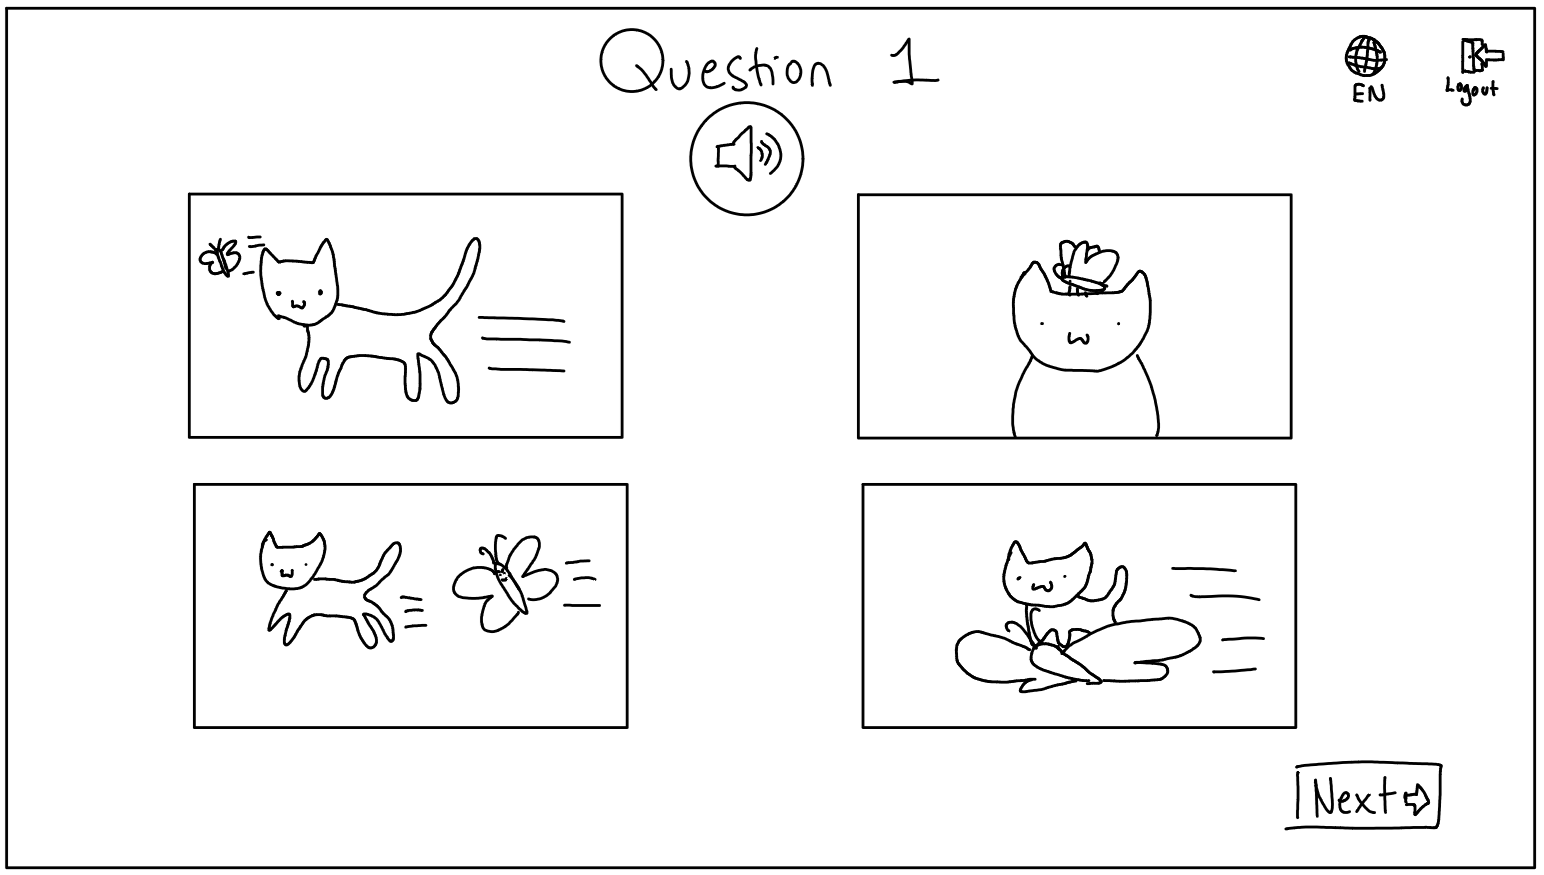
\includegraphics[width=0.75\textwidth]{images/ExampleQuestion.png}
  \caption{Sketch of Example Question Page}
  \label{figEQ}
\end{figure}

\begin{figure}[H]
  \centering
  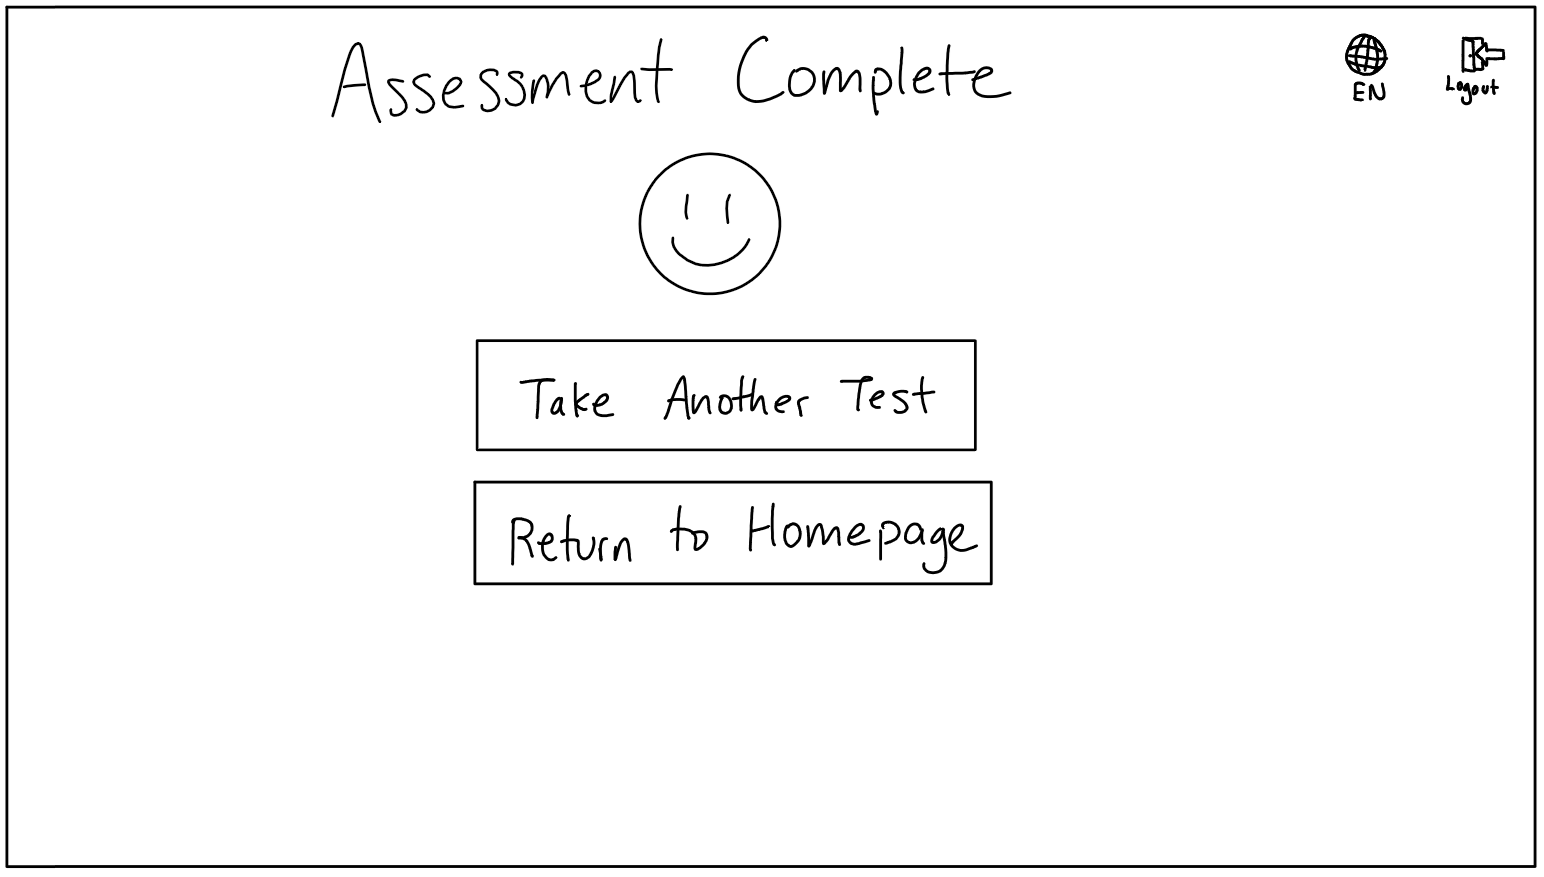
\includegraphics[width=0.75\textwidth]{images/TestComplete.png}
  \caption{Sketch of Assessment Completion Page}
  \label{figAC}
\end{figure}

\newpage

\hspace{1.5em}The below finite state machine depicts how the overall system can be interacted with, as well as which actions lead to changes in states in the system. Included in this Finite State Machine
              are Clinician Dashboard and Assessment, which are further expanded in Figure 20 and Figure 21.
\begin{figure}[H]
  \centering
  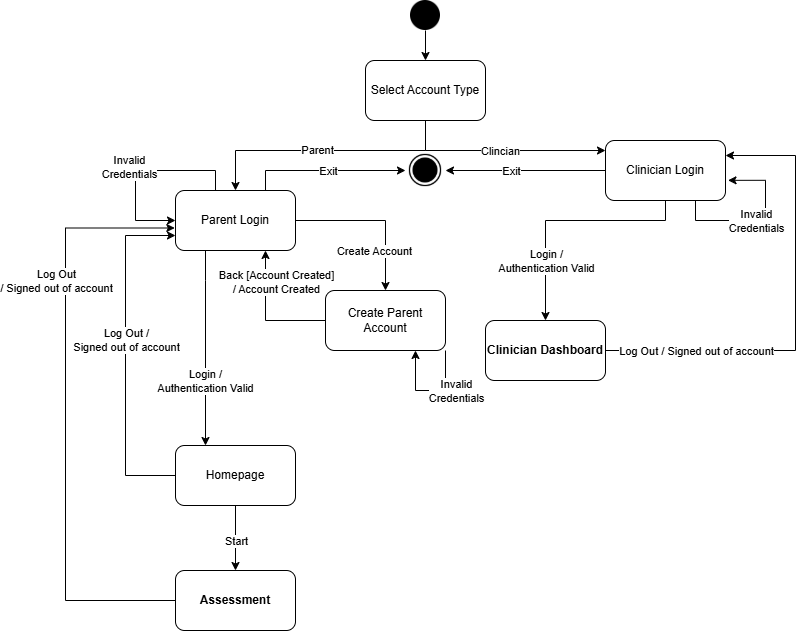
\includegraphics[scale=0.6]{images/state_diagram.drawio.png}
  \caption{FSM - TeleHealth Insights System}
\end{figure}

\newpage

\hspace{1.5em}The below finite state machine depicts how the clinician can interface with the dashboard, as well as which interactions lead to changes in states in the system.
\begin{figure}[H]
  \centering
  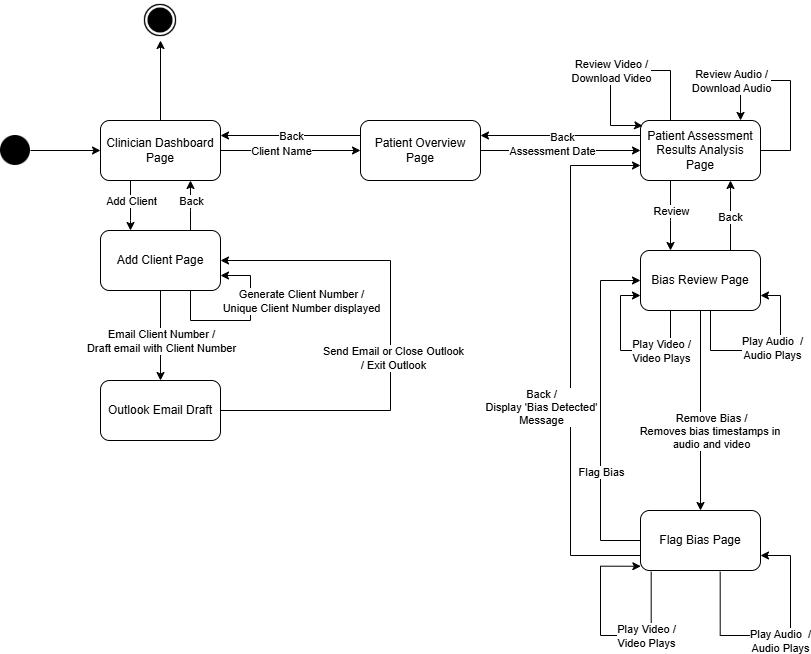
\includegraphics[scale=0.6]{images/FSM_Clinician_Dashboard.png}
  \caption{FSM - Clinician Dashboard}
\end{figure}

\newpage

\hspace{1.5em}The below finite state machine depicts how the parent and child can interface with the assessment, as well as which interactions lead to changes in states in the system.
\begin{figure}[H]
  \centering
  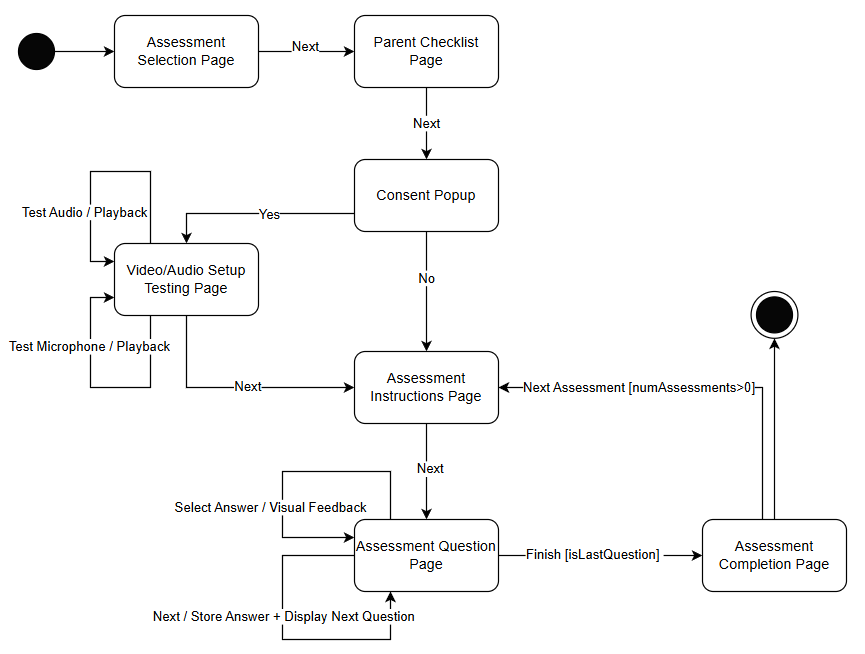
\includegraphics[scale=0.6]{images/FSM_Assessment.png}
  \caption{FSM - Assessment Dashboard}
\end{figure}

\newpage

\section{Design of Communication Protocols}

N/A

\newpage
\begin{landscape}
\section{Timeline}
\scriptsize
\begin{longtable}{|c|c|c|c|c|c|c|c|}
  \hline
      \textbf{Milestone} & \textbf{Module/Pages} & \textbf{Objective} & \textbf{Mitchell} & \textbf{Parisha} & \textbf{Promish} & \textbf{Jasmine} & \textbf{Date} \\ \hline
      Controllers & API Gateway & ~ & ~ & ~ & X & ~ & 1/19/25 \\ \hline
      Assessment & Question Bank Module & ~ & X & X & ~ & ~ & 1/19/25 \\ \hline
      Assessment & English Question Bank  Module & ~ & X & X & ~ & ~ & 1/19/25 \\ \hline
      Assessment & Matching Question Bank  Module & ~ & X & X & ~ & ~ & 1/19/25 \\ \hline
      Assessment & Repetition Question Bank  Module & ~ & X & X & ~ & ~ & 1/19/25 \\ \hline
      Assessment & ~ & Verification and Validation Testing & X & X & X & X & 1/19/25 \\ \hline
      Assessment GUI & Assessment Selection Page & ~ & ~ & ~ & ~ & X & 1/19/25 \\ \hline
      Assessment GUI & Parent Checklist Page & ~ & ~ & X & ~ & ~ & 1/22/25 \\ \hline
      Assessment GUI & Input Check Page & ~ & ~ & ~ & ~ & X & 1/22/25 \\ \hline
      Assessment GUI & Assessment Questions Page & ~ & X & ~ & ~ & ~ & 1/22/25 \\ \hline
      Clinician Dashboard & Result Storage Module & ~ & ~ & ~ & X & ~ & 1/22/25 \\ \hline
      Assessment GUI & Assessment Instructions Page & ~ & ~ & X & ~ & ~ & 1/25/25 \\ \hline
      Assessment GUI & Tutorial Page & ~ & X & ~ & ~ & ~ & 1/25/25 \\ \hline
      Assessment GUI & Assessment Completion Page & ~ & ~ & ~ & ~ & X & 1/25/25 \\ \hline
      Assessment GUI & ~ & Verification and Validation Testing & X & X & X & X & 1/25/25 \\ \hline
      Clinician Dashboard & Report Generation Module & ~ & ~ & ~ & X & ~ & 1/25/25 \\ \hline
      Clinician Dashboard & ~ & Verification and Validation Testing & X & X & X & X & 1/25/25 \\ \hline
      Clinician Dashboard GUI & Clinician Dashboard Overview Page & ~ & X & ~ & ~ & ~ & 1/28/25 \\ \hline
      Clinician Dashboard GUI & Patient Overview Page & ~ & ~ & X & ~ & ~ & 1/28/25 \\ \hline
      Clinician Dashboard GUI & Patient Assessment Results Analysis Page & ~ & ~ & ~ & ~ & X & 1/28/25 \\ \hline
      Media Processing & Media Processing Module & ~ & ~ & ~ & X & ~ & 1/28/25 \\ \hline
      Clinician Dashboard GUI & Bias Review Page & ~ & ~ & ~ & ~ & X & 1/31/25 \\ \hline
      Clinician Dashboard GUI & Add New Client Page & ~ & X & ~ & ~ & ~ & 1/31/25 \\ \hline
      Clinician Dashboard GUI & ~ & Verification and Validation Testing & X & X & X & X & 1/31/25 \\ \hline
      Homepage & Authentication Module & ~ & ~ & ~ & X & ~ & 1/31/25 \\ \hline
      Homepage GUI & Select Account Type Page & ~ & ~ & X & ~ & ~ & 1/31/25 \\ \hline
      Homepage GUI & Login Page (Parent) Page & ~ & ~ & X & ~ & ~ & 2/3/25 \\ \hline
      Homepage GUI & Login Page (Clinician) Page & ~ & ~ & X & ~ & ~ & 2/3/25 \\ \hline
      Homepage GUI & Create Account Page & ~ & X & ~ & ~ & ~ & 2/3/25 \\ \hline
      Homepage GUI & Homepage (Parent) Page & ~ & ~ & ~ & ~ & X & 2/3/25 \\ \hline
      Homepage GUI & ~ & Verification and Validation Testing & X & X & X & X & 2/3/25 \\ \hline
      Media Processing & Video Processing Module & ~ & ~ & ~ & X & ~ & 2/3/25 \\ \hline
      Media Processing & Audio Processing Module & ~ & X & ~ & ~ & ~ & 2/6/25 \\ \hline
      Media Processing & ~ & Verification and Validation Testing & X & X & X & X & 2/6/25 \\ \hline
      Miscellaneous & Logging Module & ~ & ~ & X & ~ & ~ & 2/6/25 \\ \hline
      Miscellaneous & Real-Time Feedback Module & ~ & ~ & ~ & X & ~ & 2/6/25 \\ \hline
      Miscellaneous & ~ & Verification and Validation Testing & X & X & X & X & 2/6/25 \\ \hline
      Admin & Add Clinician Page & ~ & ~ & ~ & ~ & X & 2/6/25 \\ \hline
      Admin & ~ & Verification and Validation Testing & X & X & X & X & 2/6/25 \\ \hline
      Controllers & Landing Page GUI & ~ & ~ & ~ & X & ~ & 1/19/25 \\ \hline
      Controllers & ~ & Verification and Validation Testing & X & X & X & X & 1/19/25 \\ \hline
      Rev0 & ~ & Full System Testing & X & X & X & X & 2/8/25 \\ \hline
      Rev0 & ~ & Rev0 Practice & X & X & X & X & 2/9/25 \\ \hline
      Rev0 & ~ & Rev0 Presentation & X & X & X & X & 2/10/25 \\ \hline
\end{longtable}
\normalsize
\end{landscape}

\bibliographystyle {plainnat}
\bibliography{../../../refs/References}

\newpage{}

\end{document}